\documentclass{beamer}
\usepackage{comment}
\usepackage{multirow}
\usepackage{bibentry}
\usepackage{booktabs}
\usepackage{amsmath}
\usepackage[utf8]{inputenc}
\graphicspath{ {./images/} }

%Information to be included in the title page:
\title{Model Robustness Isn’t Security}
\author{Sven Cattell}
\date{Bsides LV, 2022}

\AtBeginSection[]
{
  \begin{frame}
    \frametitle{Table of Contents}
    \tableofcontents[currentsection]
  \end{frame}
}

\begin{document}

\frame{\titlepage}
\begin{frame}
\frametitle{About Me}
\begin{itemize}
\item Founded a startup in this space, still in stealth
\item Ph.D. in Algebraic Topology from JHU
\item Very involved in the AI Village
\item Formerly at Endgame / Elastic
\end{itemize}
\end{frame}

\begin{frame}
\frametitle{Table of Contents}
\tableofcontents
\end{frame}

\section{The Need for Definitions}

\begin{frame}
    \frametitle{The Adversarial Example Definition Everyone Says}
    \textbf{OpenAI} - Adversarial examples are inputs to machine learning models that an attacker has intentionally designed to cause the model to make a mistake; they're like optical illusions for machines.
    \newline
    \newline
    \textbf{TensorFlow} - Adversarial examples are specialised inputs created with the purpose of confusing a neural network, resulting in the misclassification of a given input.
\end{frame}

\begin{frame}
    \frametitle{The Problems with the Adversarial Example Definitions Everyone Says}
    \begin{enumerate}
        \item Any model error can fit the definition, if you squint.
        \item This is not close to the definition practitioners mean.
        \item If you use this definition, people can sell you snake oil that does nothing.
        \item Even if you use the correct definition, people can sell you snake oil that does nothing.
    \end{enumerate}
\end{frame}

\begin{frame}
    \frametitle{The Robust Definition Everyone Says}
    \textbf{Investopedia} - In the world of investing, robust is a characteristic describing a model's, test's, or system's ability to perform effectively while its variables or assumptions are altered.
    \newline
    \newline
    \textbf{Data Robot} - A way of modeling that to minimizes your productionalized model from uncertain predictions.
\end{frame}

\begin{frame}
    \frametitle{The Problems with the Robust Definitions Everyone Says}
    \begin{enumerate}
        \item Both definitions just mean you have a good model that generalizes.
        \item This lets them check by wiggling some minor parameters, not actually testing the model on new data.
    \end{enumerate}
\end{frame}

\begin{frame}
    \frametitle{Terms you Need to Navigate this space}
    \begin{enumerate}
        \item \textbf{Neighborhood} - a ball around a point.
        \item \textbf{Adversarial Example} - a point in a \textit{small neighborhood} of a sample that has a different classification than the sample with your classification function.
        \item \textbf{Point Cloud} - The set of all points in your training set. 
        \item \textbf{Distribution} - the underlying process that generates samples that are in your \textit{point cloud}.
        \item \textbf{Robust} - If a new point is introduced within a neighborhood of an in-distribution point, it will be classified the same way.
    \end{enumerate}
\end{frame}

\section{What's a Neighborhood}

\begin{frame}
    \frametitle{What's a Neighborhood}
    There are many ways of calculating "distance" and this impacts the problem in subtle ways.
    $$\text{Dist}_2(x, y) = ||x - y||_2 = \sqrt{ \sum_{i=1}^{k} (x_i - y_i)^2}$$  
    $$\text{Dist}_\infty(x, y) = ||x - y||_\infty = \max_{{i \in \{1, 2, \dots k\}}} |x_i - y_i| $$
    A neighborhood of a point is all points within some chosen $\delta$ of your point:
    $$\text{Ball}_2^\delta(x) = \lbrace y \in \mathbb{R}^k ~~ \text{s.t.} ~~ ||x-y||_2 < \delta \rbrace $$  
    $$\text{Ball}_\infty^\delta(x) = \lbrace y \in \mathbb{R}^k ~~ \text{s.t.} ~~ ||x-y||_\infty < \delta \rbrace $$  

\end{frame}

\begin{frame}
    \frametitle{Dimensions are weird, 1: String around the Earth}
    How much more rope do we need to wrap a rope around the earth that is 1 foot above the ground than one that wraps exactly?
    \begin{center}
    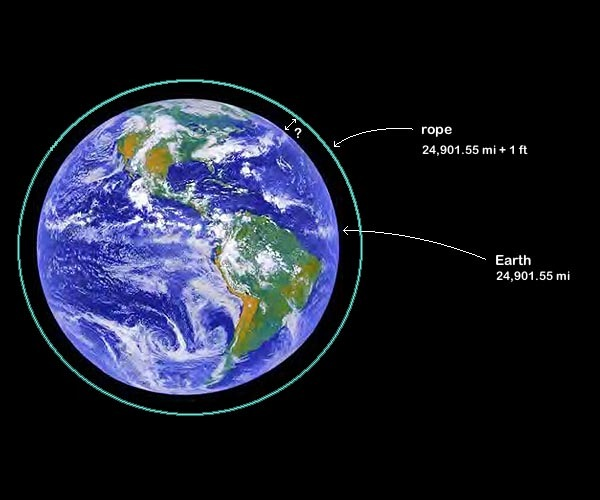
\includegraphics[scale=0.4]{Rope_around_earth_3.jpg}
    \end{center}
\end{frame}

\begin{frame}
    \frametitle{Dimensions are weird, 2: Square Cubed Law}
    If $h$ is the height of a solid then the surface area grows with $O(h^2)$ and the volume grows with $O(h^3)$. Elephant ears combat this:
    \begin{center}
    \includegraphics[scale=0.04]{Elephant_Diversity.jpg}
    \end{center}
\end{frame}

\begin{frame}
    \frametitle{Dimensions are weird, 3: Sphere Packing}
    In dimension $d$ inscribe $2^d$ $d$-spheres in the unit $d$-cube. Then inscribe a $d$-sphere that just touches each of the $d$-spheres.

    What happens to the center sphere as we increase $d$?
    \begin{center}
    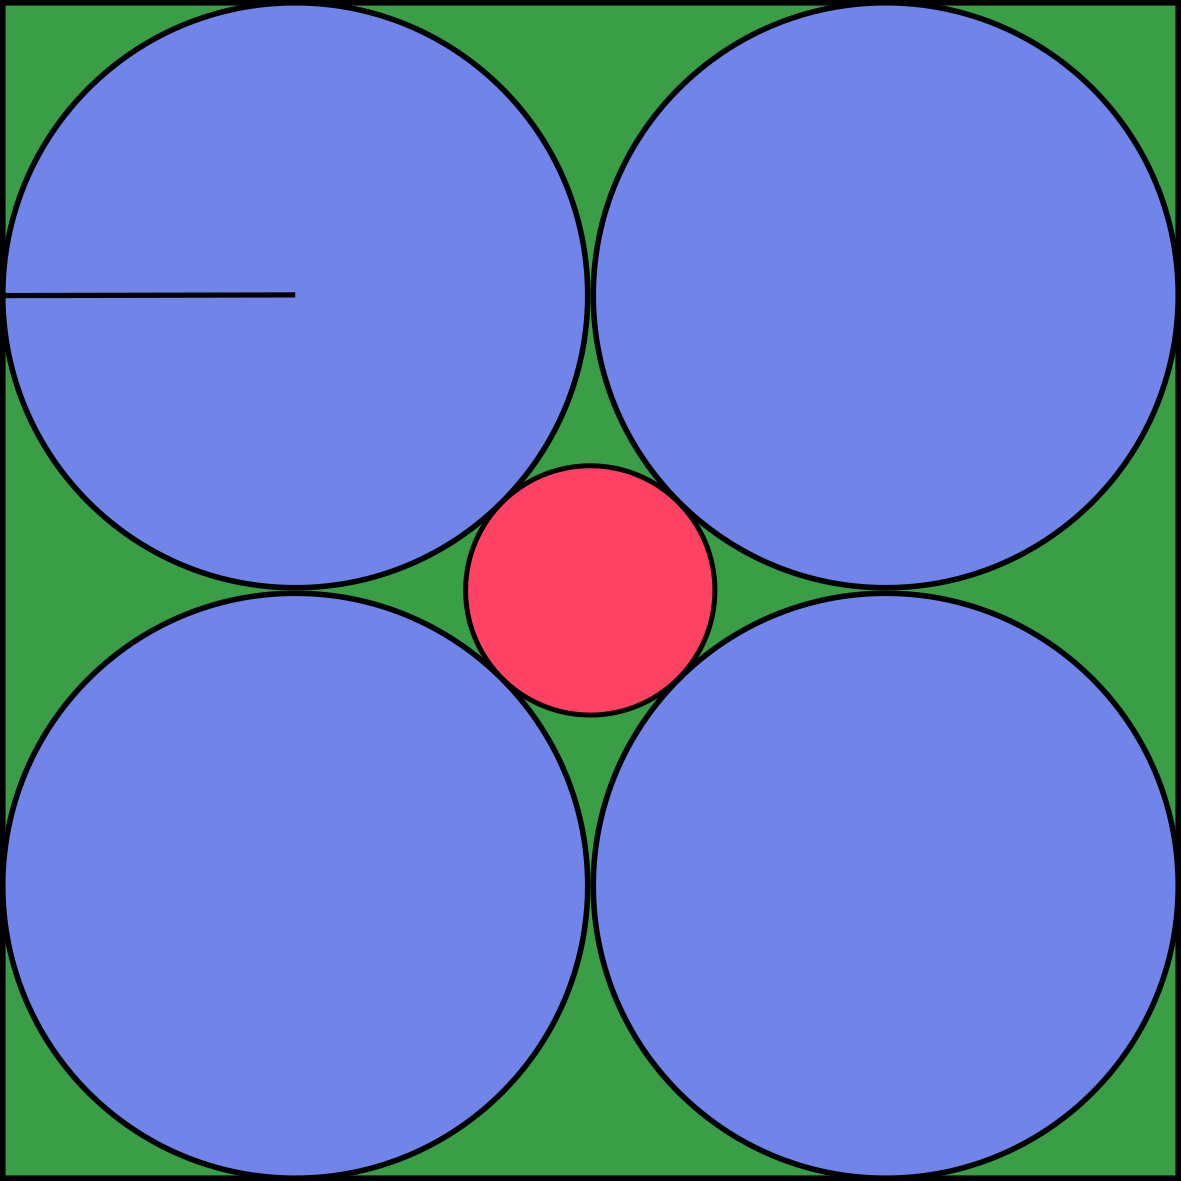
\includegraphics[scale=0.7]{sphere_illustration.png}

    Mathematicians get this wrong!
    \end{center}
\end{frame}

\begin{frame}
    \frametitle{Dimensions are weird, 4: MNIST Degrees of Freedom}
    Each MNIST digit is a square image of 28x28 8-bit pixels, so each pixel is one of 256 values. If I am allowed to perturb each pixel in the image by 1 value I have $$3^{(24^2)}=3^{784} \thickapprox 2^{1242}$$ possible perturbations.
    \begin{center}
    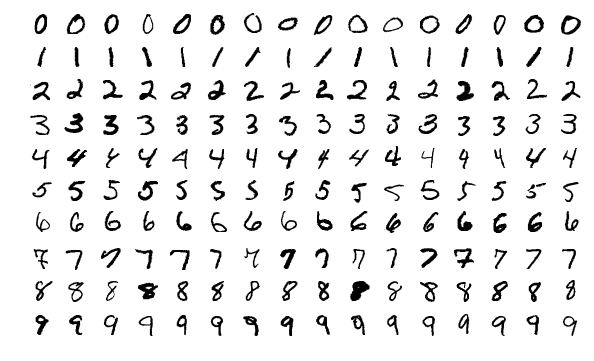
\includegraphics[scale=0.42]{MnistExamples.png}
    \end{center}
\end{frame}

\begin{frame}
    \frametitle{What's a Neighborhood: Takeaways}
    \begin{enumerate}
        \item The volume of high dimensional neighborhoods grows exponentially with the dimension.
        \item This messes up machine learning and is known as the \textbf{Curse of Dimensionality}.
    \end{enumerate}
\end{frame}

\section{Defining Adversarial Examples \& Robustness}

\begin{frame}
    \frametitle{The Legally Required Panda-Gibbon}
    \begin{center}
    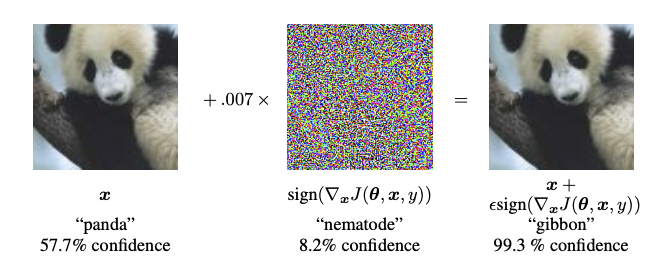
\includegraphics[scale=0.45]{adversarial_example.png}
    \end{center}
    \cite{fgsm_paper}
\end{frame}

\begin{frame}
    \frametitle{A Definition for Adversarial Examples}
    \begin{center}
    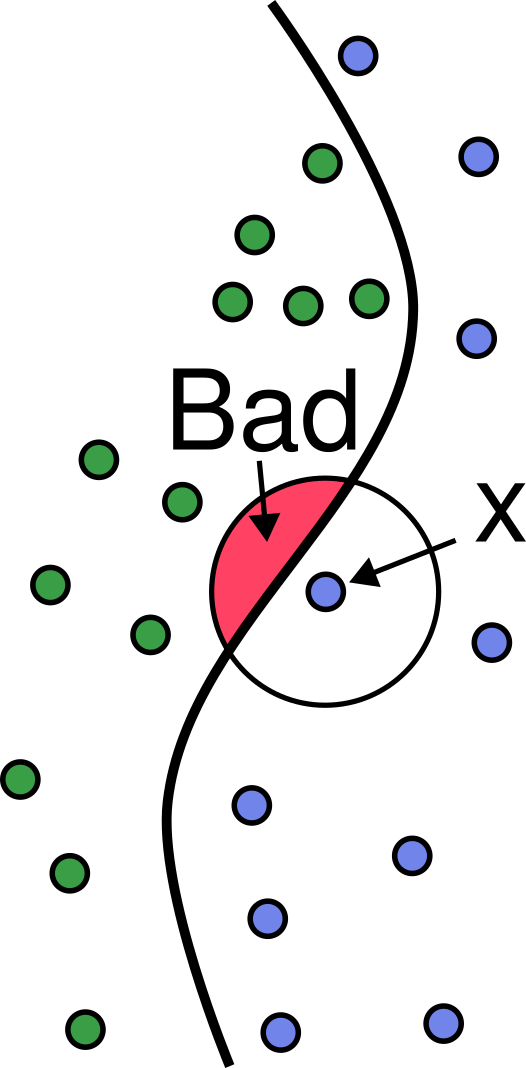
\includegraphics[scale=1.1]{current_definition.png}
    \end{center}
    Any input within a small ball around our target point that changes the output is an adversarial example for that target point.
\end{frame}

\begin{frame}
    \frametitle{Fully Formal Definition of Adversarial Examples}
    \begin{definition}
        For  
        \begin{enumerate}
            \item a classifier $f : \mathbb{R}^m \to \{ 1, \dots k \}$,
            \item a point $x \in \mathbb{R}^m$,
            \item and a target label $l \in \{ 1, \dots k \}$
        \end{enumerate}
          
        An \textbf{adversarial example} for $x$ with target $l$ within radius $\delta$ is any $y \in [0,1]^m$ such that, 
        \begin{enumerate}
            \item $||x - y||_2 < \delta$,
            \item $f(y) = l$.
        \end{enumerate}
    \end{definition}
\end{frame}

\begin{frame}
    \frametitle{Robustness}
    \begin{definition}
        A model $f$ is $\delta$ robust on a set of points $X$ if for all $x \in X$ and $r \in \mathbb{R}^n$ such that $||r||_2 < \delta$, then:
        $$f(x) = f(x + r)$$
    \end{definition}
    \begin{center}
        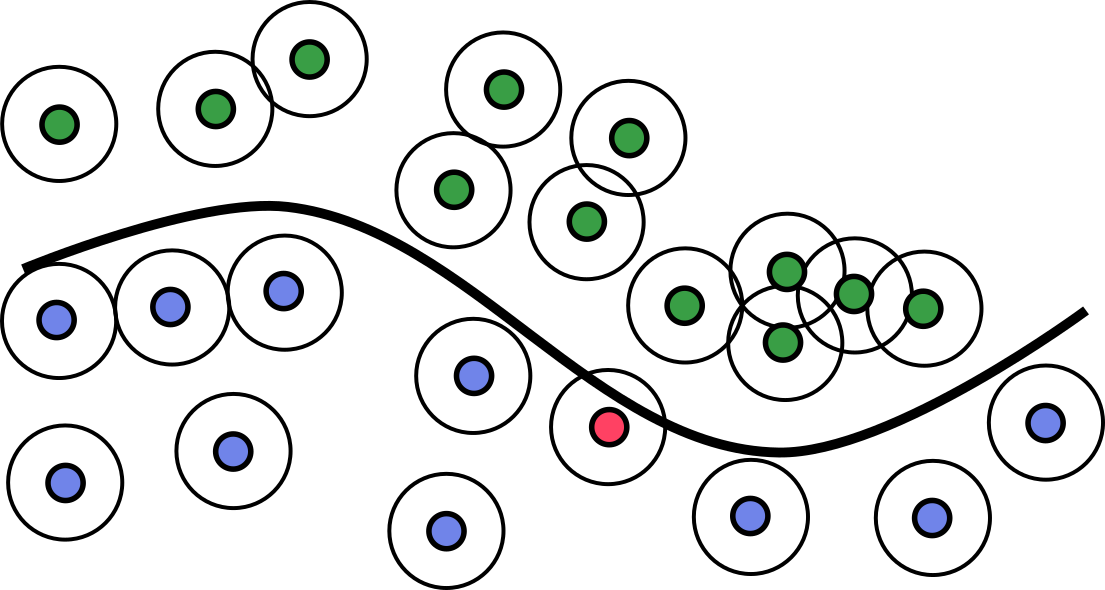
\includegraphics[scale=1.2]{robustness.png}

        The red point makes this "model" not robust with the given radius.
    \end{center}
\end{frame}

\section{The Issues with Adversarial Examples \& Robustness}

\begin{frame}
    \frametitle{The Issue with Robustness}
    \begin{center}
        1. Data Just Moves

        \vspace*{30pt}
        2. It's Impossible to Check
    \end{center}
\end{frame}


\begin{frame}
    \frametitle{The Issue with Robustness: Data just moves}
    \begin{center}
        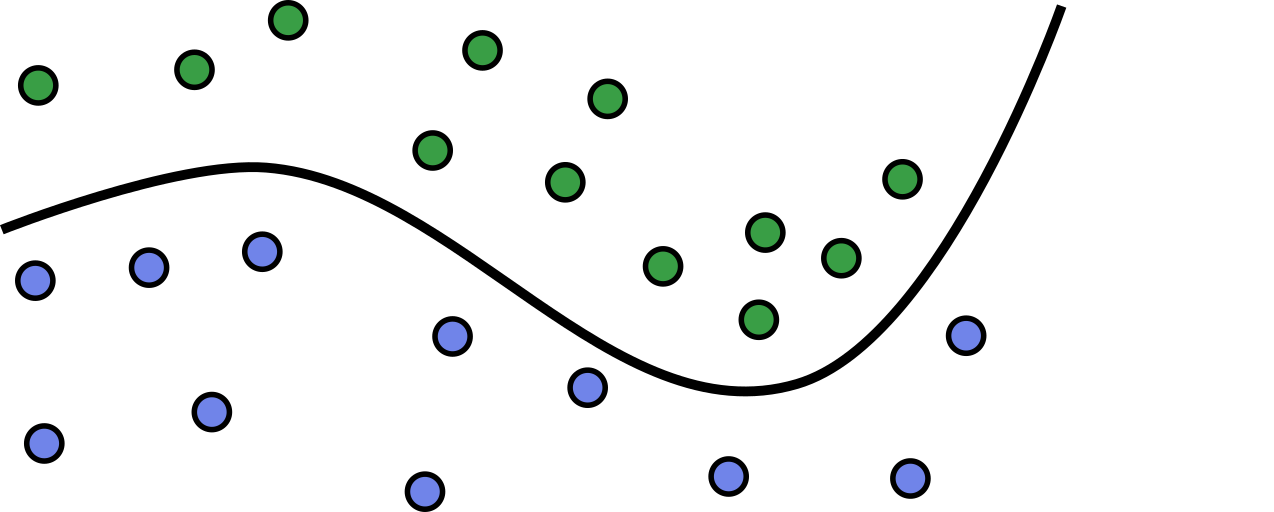
\includegraphics[scale=1.2]{training_1.png}

        We can train a robust model on the green and blue points. 

        \vspace*{20pt}
        Think of this as all the data collected up until you have to train and deploy the robust model.
    \end{center}
\end{frame}

\begin{frame}
    \frametitle{The Issues with Robustness: Data just moves}
    \begin{center}
        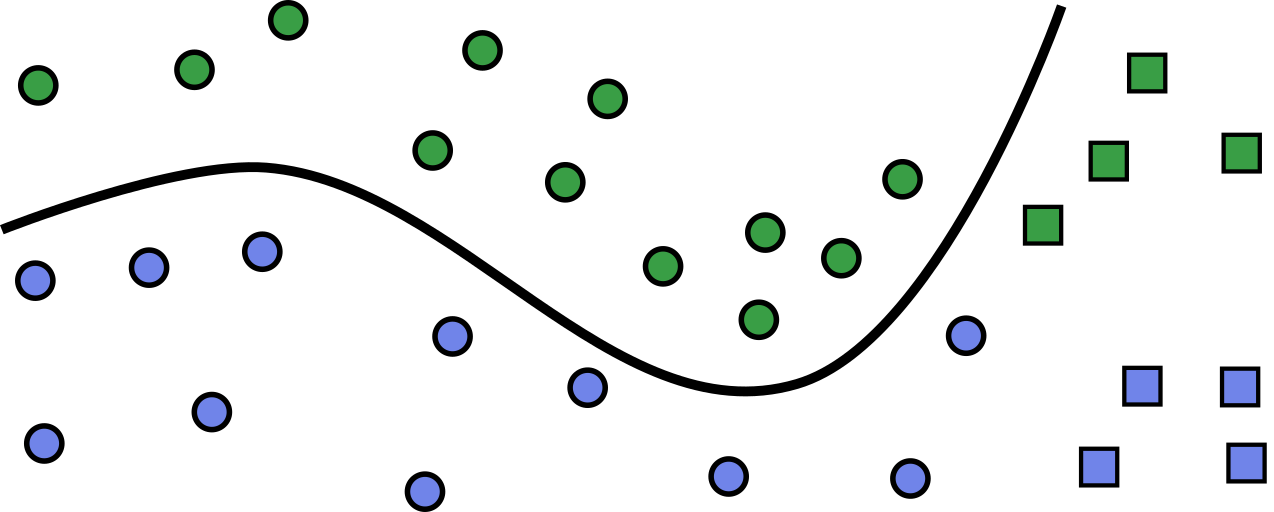
\includegraphics[scale=1.2]{training_2.png}

        A month later there's more data. 
        
        \vspace*{20pt}
        And... your robust model misclassifies the new green points as blue. 
    \end{center}
\end{frame}

\begin{frame}
    \frametitle{The Issues with Robustness: Data just moves}
    \begin{center}
        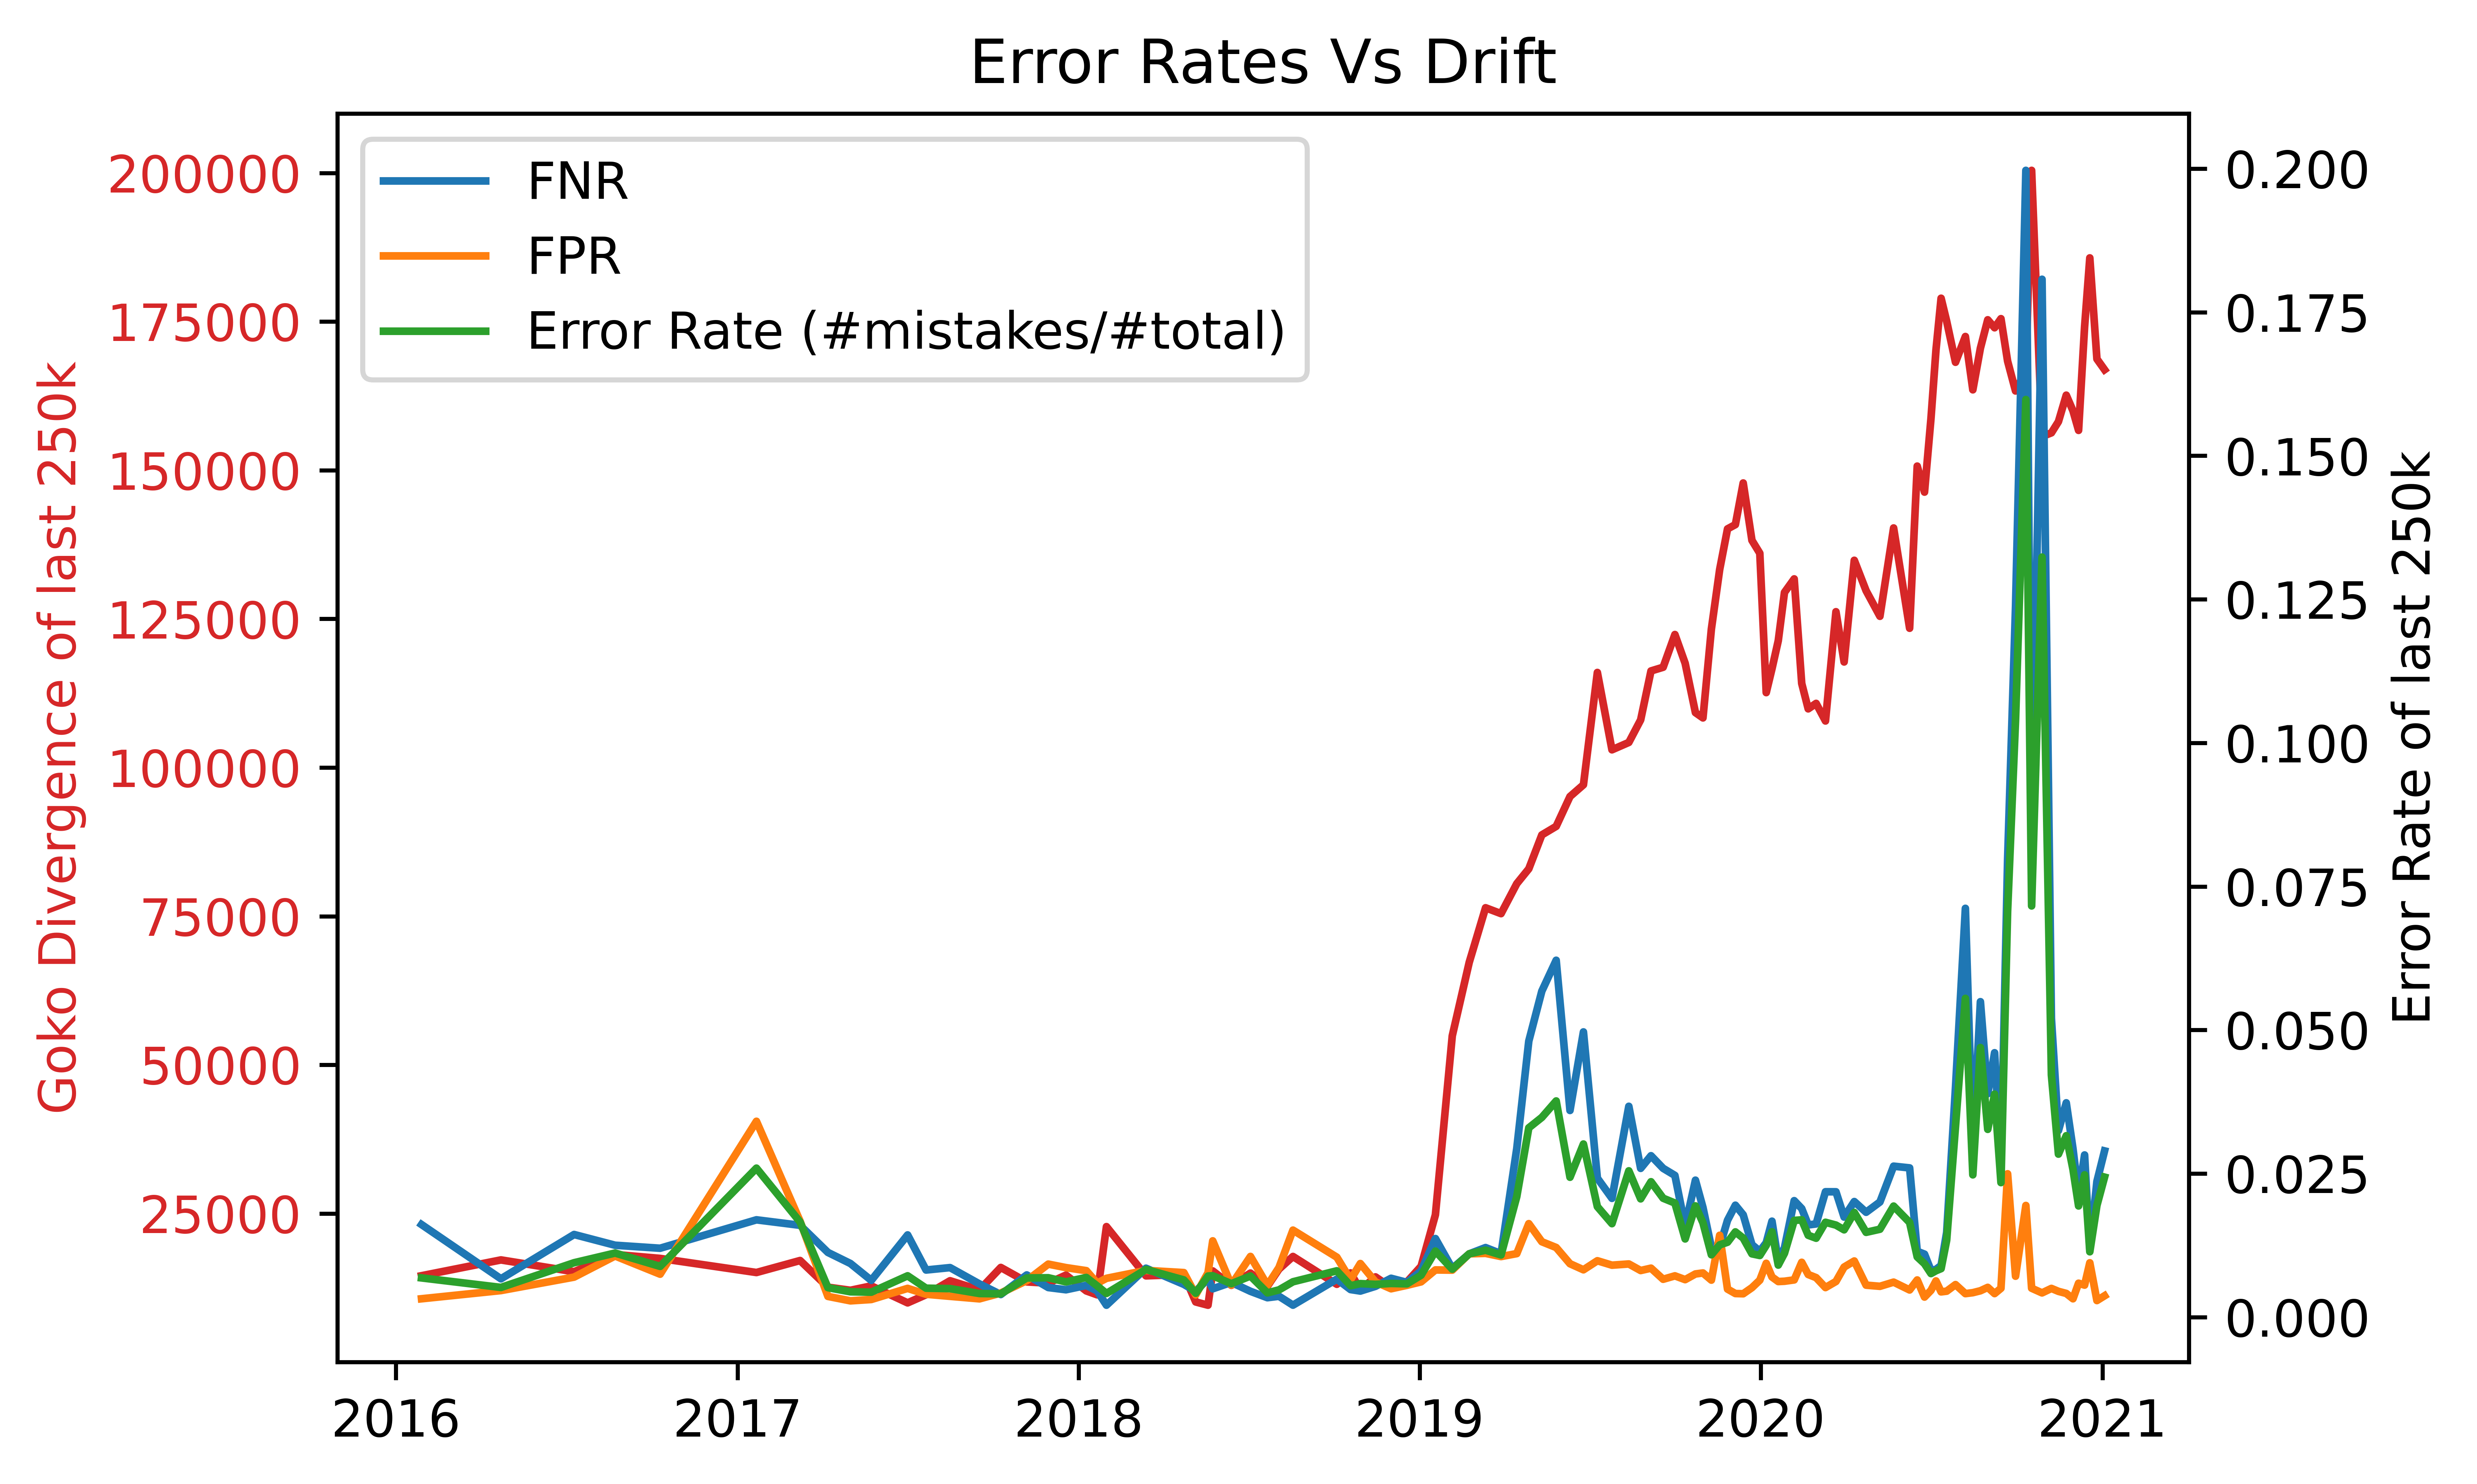
\includegraphics[scale=0.6]{overall_vs_error.png}

        This is a model trained on malware data up until 01/01/2019. The error rates (legend + axis on right) explode in March. \cite{BayesianCovertreeICLR}
    \end{center}
\end{frame}

\begin{frame}
    \frametitle{The Issues with Robustness: It's Impossible to Check}
    An MNIST model $f$ is $\delta$ robust asserts that they know that the model does the correct thing for each input.

    \vspace{10pt}
    The volume of space checked can be converted into a measure of information familiar to hackers, bits:
    
    \begin{center}
        \begin{tabular}{| c || c | c |}
            \hline
            $\delta$ & \multicolumn{2}{|c|}{Maximum Bits of Information} \\
            \hline
            & MNIST $L_2$ & MNIST $L_\infty$ \\
            \hline
        
            1 & 10.6 & \textbf{1242.6} \\
            2 & 37.9 & 1820.4 \\
            3 & 77.0 & 2201.0 \\
            4 & 125.4 & 2485.2 \\
            5 & 181.1 & 2712.2 \\
            6 & 242.9 & 2901.1 \\
            7 & \textbf{309.3} & 3063.0 \\
            8 & 379.5 & 3204.6 \\
        \hline
        \end{tabular}
    \end{center}
\end{frame}

\begin{frame}{The Issues with Robustness: It's Impossible to Check}
    \begin{center}
    So, with a radius of 7 for a MNIST, a brute force check for the $L_2$ ball needs more compute than brute forcing AES Encryption with 256bit keys. 
    
    \vspace{10pt}
    \textbf{The radius is normally more than 70.}

    \vspace{10pt}
    A smarter check may use the geometry of the neural network to check, but at that radius all bets are off.
    \end{center}
\end{frame}

\begin{frame}{The Issues with Robustness: It's Impossible to Check}
    \begin{center}
        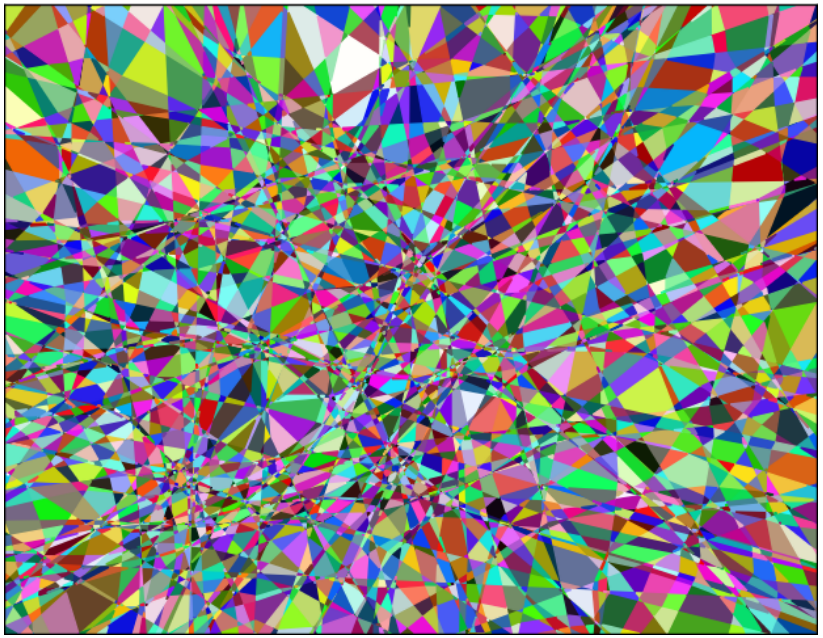
\includegraphics[scale=0.23]{image_of_2d_regions_in_mnist.png}

        A 2D slice of a neural network trained on MNIST. 
        
        Each colored polygon is a linear region in MNIST. \cite{estimate_of_linear_regions}
    \end{center}
\end{frame}

\begin{frame}{The Issues with Robustness: It's Impossible to Check}
    Using Hanin and Rolnick's estimates the bits needed to search on a reasonable network for MNIST is:
    \begin{center}
        \begin{tabular}{| c || c | c |}
            \hline
            $\delta$ & \multicolumn{2}{|c|}{Maximum Bits of Information} \\
            \hline
            & Estimate w/ H\&R & Naive Estimate \\
            \hline
                1 & 0.0 & 10.6 \\
                2 & 20.2 & 37.9 \\
                3 & 46.1 & 77.0 \\
                4 & 77.0 & 125.4 \\
                5 & 118.8 & 181.1 \\
                6 & 157.0 & 242.9 \\
                7 & 204.3 & \textbf{309.3} \\
                8 & \textbf{258.8} & 379.5 \\
            \hline
        \end{tabular}
        \vspace{10pt}

        I think we can do better than this estimate on arbitrary neural networks. I'd bet it's \textbf{closer to 128 bits} at a radius of 8.
    \end{center}
\end{frame}

\begin{frame}{The Issues with Robustness: It Lowers Accuracy}
    TODO
\end{frame}


\section{How Bypasses Really Work}

\begin{frame}{Case Study: First Major ML Attack}
    Probably the first deployment of ML in Security was in spam filtering in about 2002, using Naive Bayes \cite{spam_bayes}.
    \vspace{10pt} \pause

    By 2004 various attacks had been seen in the wild \cite{how_to_beat_spam}:
    \begin{enumerate}
        \item Obfuscating text 
        \item Small emails that just hold links
        \item Hiding the email in an Non-Deliverable Return
        \item Packing the email with "good words"
    \end{enumerate}
    \vspace{10pt} \pause

    These are not "adversarial examples" as we've been discussing. \textbf{These are people sitting down with an understanding of how your system works and figuring out a bypass.}
\end{frame}

\begin{frame}{Case Study: A Recent ML Attack}
    \begin{center}
        Elastic's EMBER's Featurization System \cite{anderson2018ember}:
        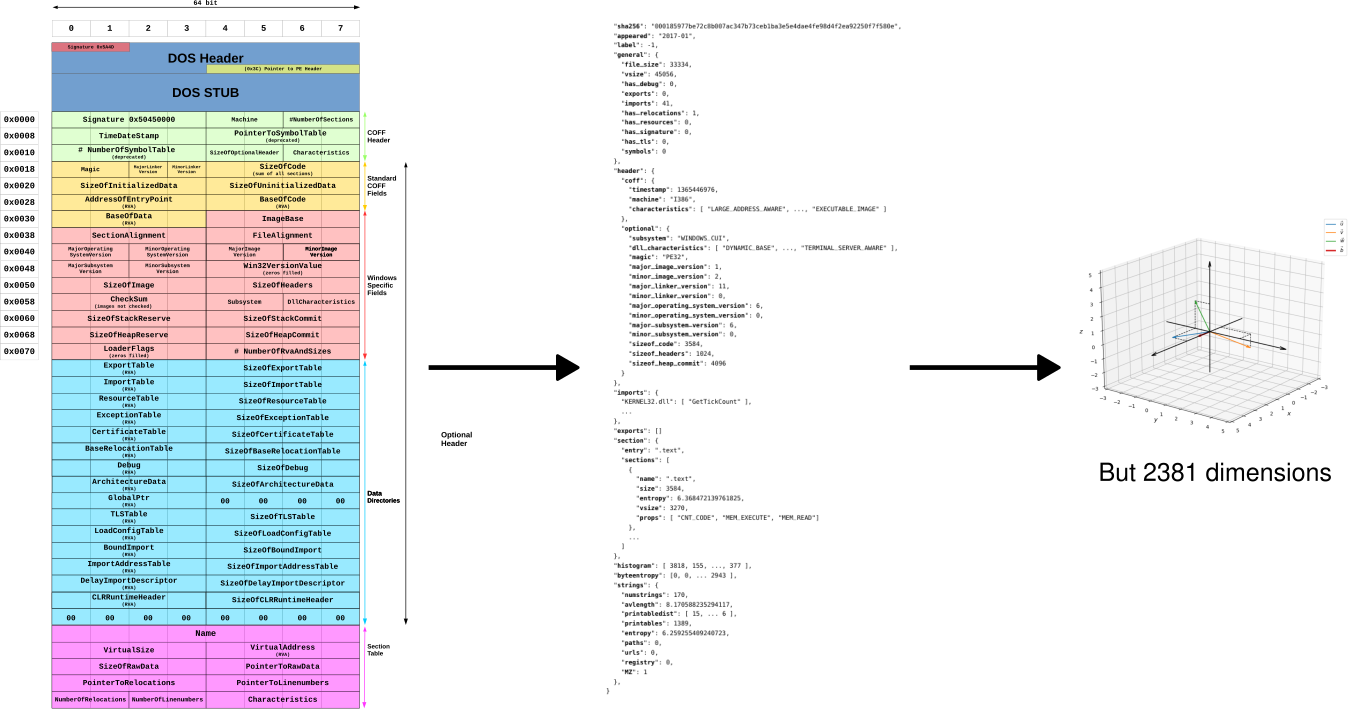
\includegraphics[scale=0.18]{ember_diagram.png}
    \end{center}
\end{frame}

\begin{frame}{Case Study: A Recent ML Attack}
    In 2019 Adi Ashkenazy and Shahar Zini reverse engineered the Cylance malware detector and found a bypass \cite{cylance_i_kill_you}.
    \vspace{10pt}
    \begin{center}
        Part of Cylance's Malware Detection System:
        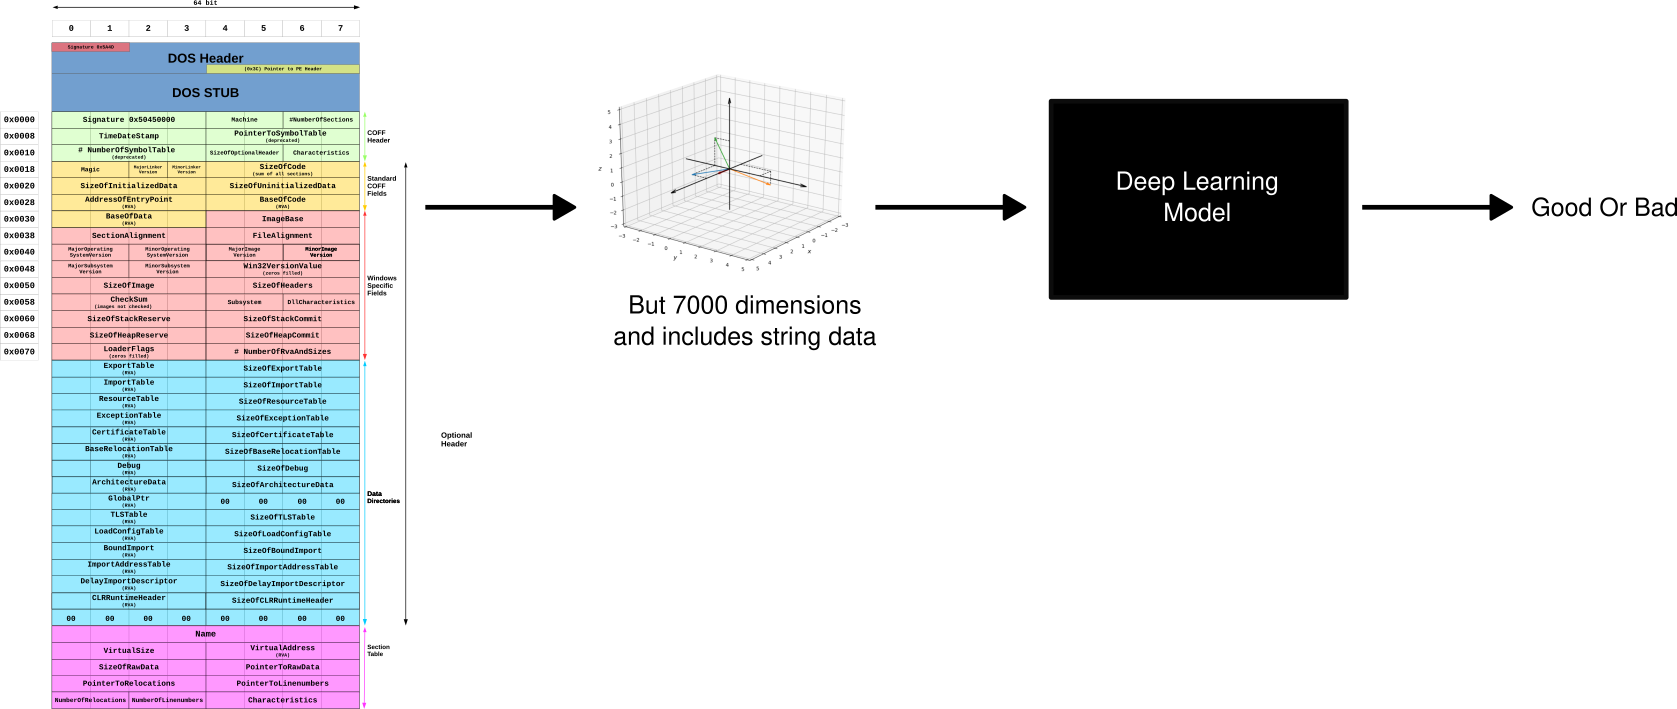
\includegraphics[scale=0.15]{cylance_diagram1.png}
    \end{center}
\end{frame}

\begin{frame}{Case Study: A Recent ML Attack}
    In 2019 Adi Ashkenazy and Shahar Zini reverse engineered the Cylance malware detector and found a bypass \cite{cylance_i_kill_you}.
    \vspace{10pt}
    \begin{center}
        Part of Cylance's Malware Detection System:
        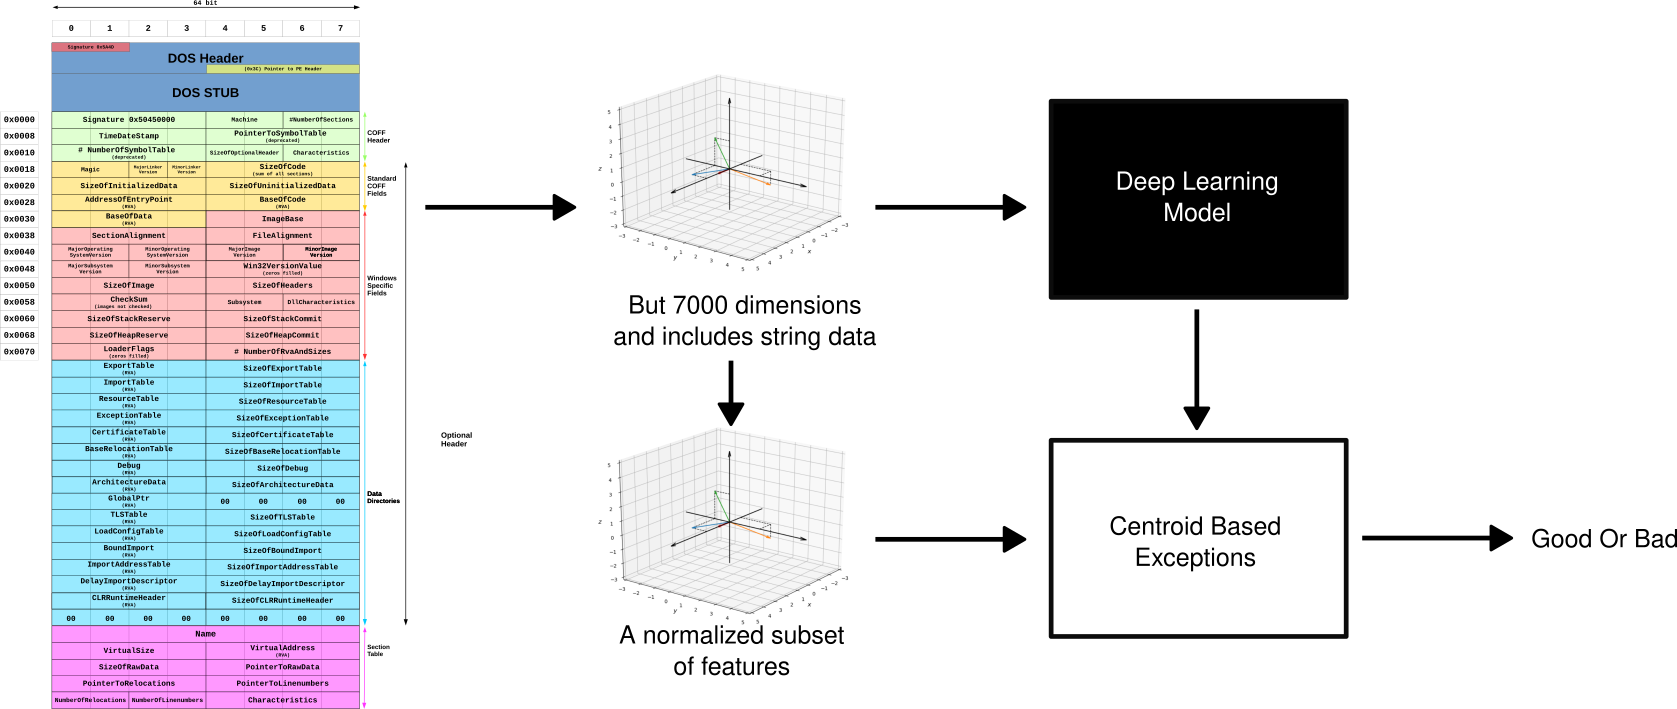
\includegraphics[scale=0.15]{cylance_diagram2.png}
    \end{center}
\end{frame}

\begin{frame}{Case Study: A Recent ML Attack}
    In 2019 Adi Ashkenazy and Shahar Zini reverse engineered the Cylance malware detector and found a bypass \cite{cylance_i_kill_you}.
    \vspace{10pt}
    \begin{center}
        Part of Cylance's Malware Detection System:
        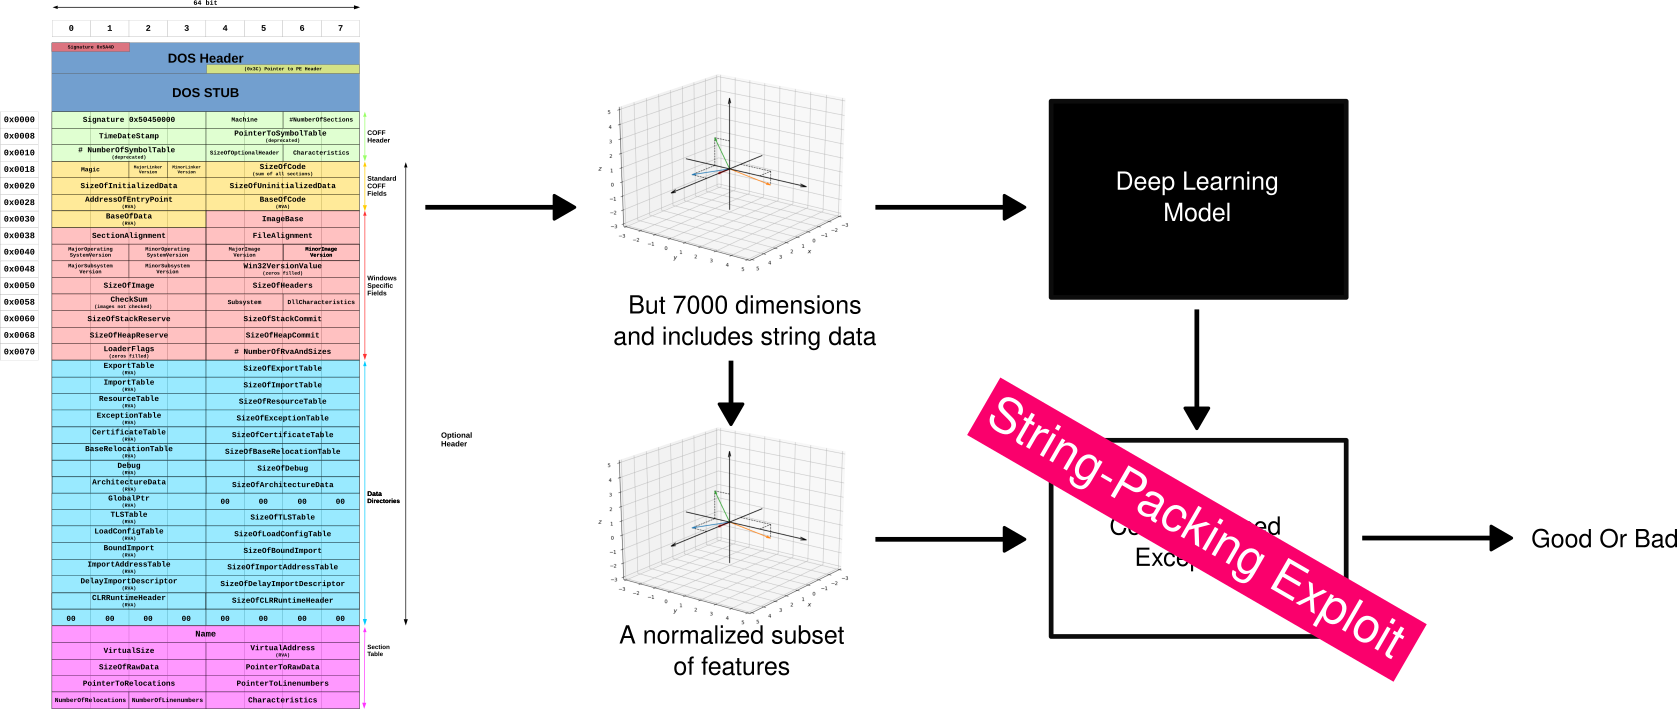
\includegraphics[scale=0.15]{cylance_diagram3.png}
    \end{center}
\end{frame}

\section{Real Security Recommendations}

\begin{frame}{Real Security: Fundamentals}
    \begin{center}
        \textbf{It's still software, do the basics!}
        \vspace{20pt}

    \end{center}
    \begin{enumerate}
        \item Validate your inputs. 
        \item Double check your pickles.
        \item Check your deployments for CVEs.
        \item Harden everything.
        \item Secure your S3 buckets.
    \end{enumerate}
\end{frame}

\begin{frame}{Real Security: Fundamentals}
    From: The Institute for Ethical AI \& Machine Learning \cite{mlsecops_10}
    \begin{enumerate}
        \item Unrestricted Model Endpoints
        \item Access to Model Artifacts 
        \item Artifact Exploit Injection 
        \item Insecure ML Systems/Pipeline Design
        \item Data \& ML Infrastructure Misconfigurations
        \item Supply Chain Vulnerabilities in ML Code
        \item IAM \& RBAC Failures for ML Services
        \item ML Infra / ETL / CI / CD Integrity Failures
        \item Observability, Reproducibility \& Lineage
        \item ML-Server Side Request Forgery
    \end{enumerate}
\end{frame}

\begin{frame}{Real Security: Dataset}
    \begin{center}
        \textbf{Your Dataset is more valuable than your model.}
        \vspace{20pt}

        Unless you're at OpenAI training GPT-5 you probably spend far more on your dataset than training your model.
        \vspace{10pt}

        You can retrain your model, change your features, and improve it, \textbf{if you have your data!}
    \end{center}
\end{frame}

\begin{frame}{Real Security: Layers}
    \begin{center}
        \textbf{Don't leave ML unattended. Treat it like a toddler.}
        \vspace{10pt}

        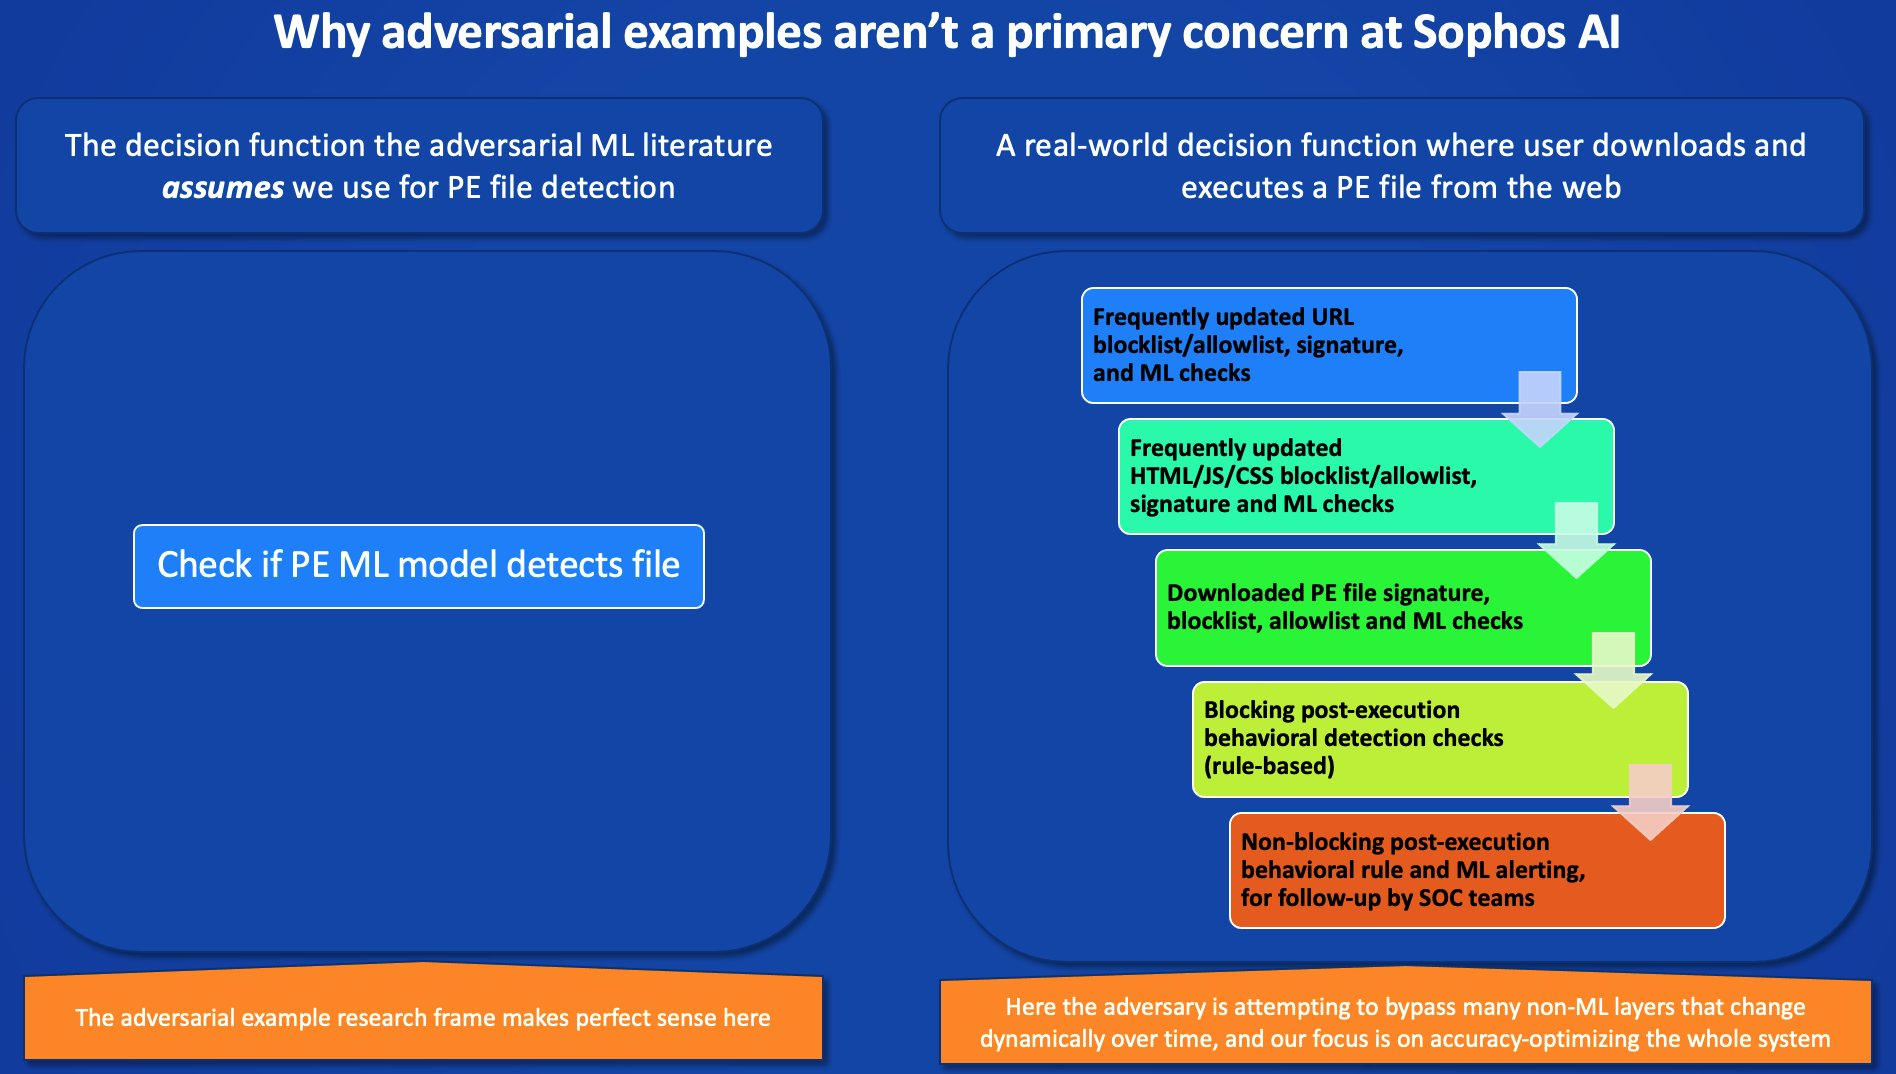
\includegraphics[scale=0.15]{sophos_ML_model.jpg}

        From Joshua Saxe's twitter, $@$joshua\_sax
    \end{center}
\end{frame}

\begin{frame}{Real Security: Understand Your Distribution}
    \begin{center}
        \textbf{Don't deploy and forget. Monitor your model! Redeploy when stale!}
        \vspace{10pt}
        
        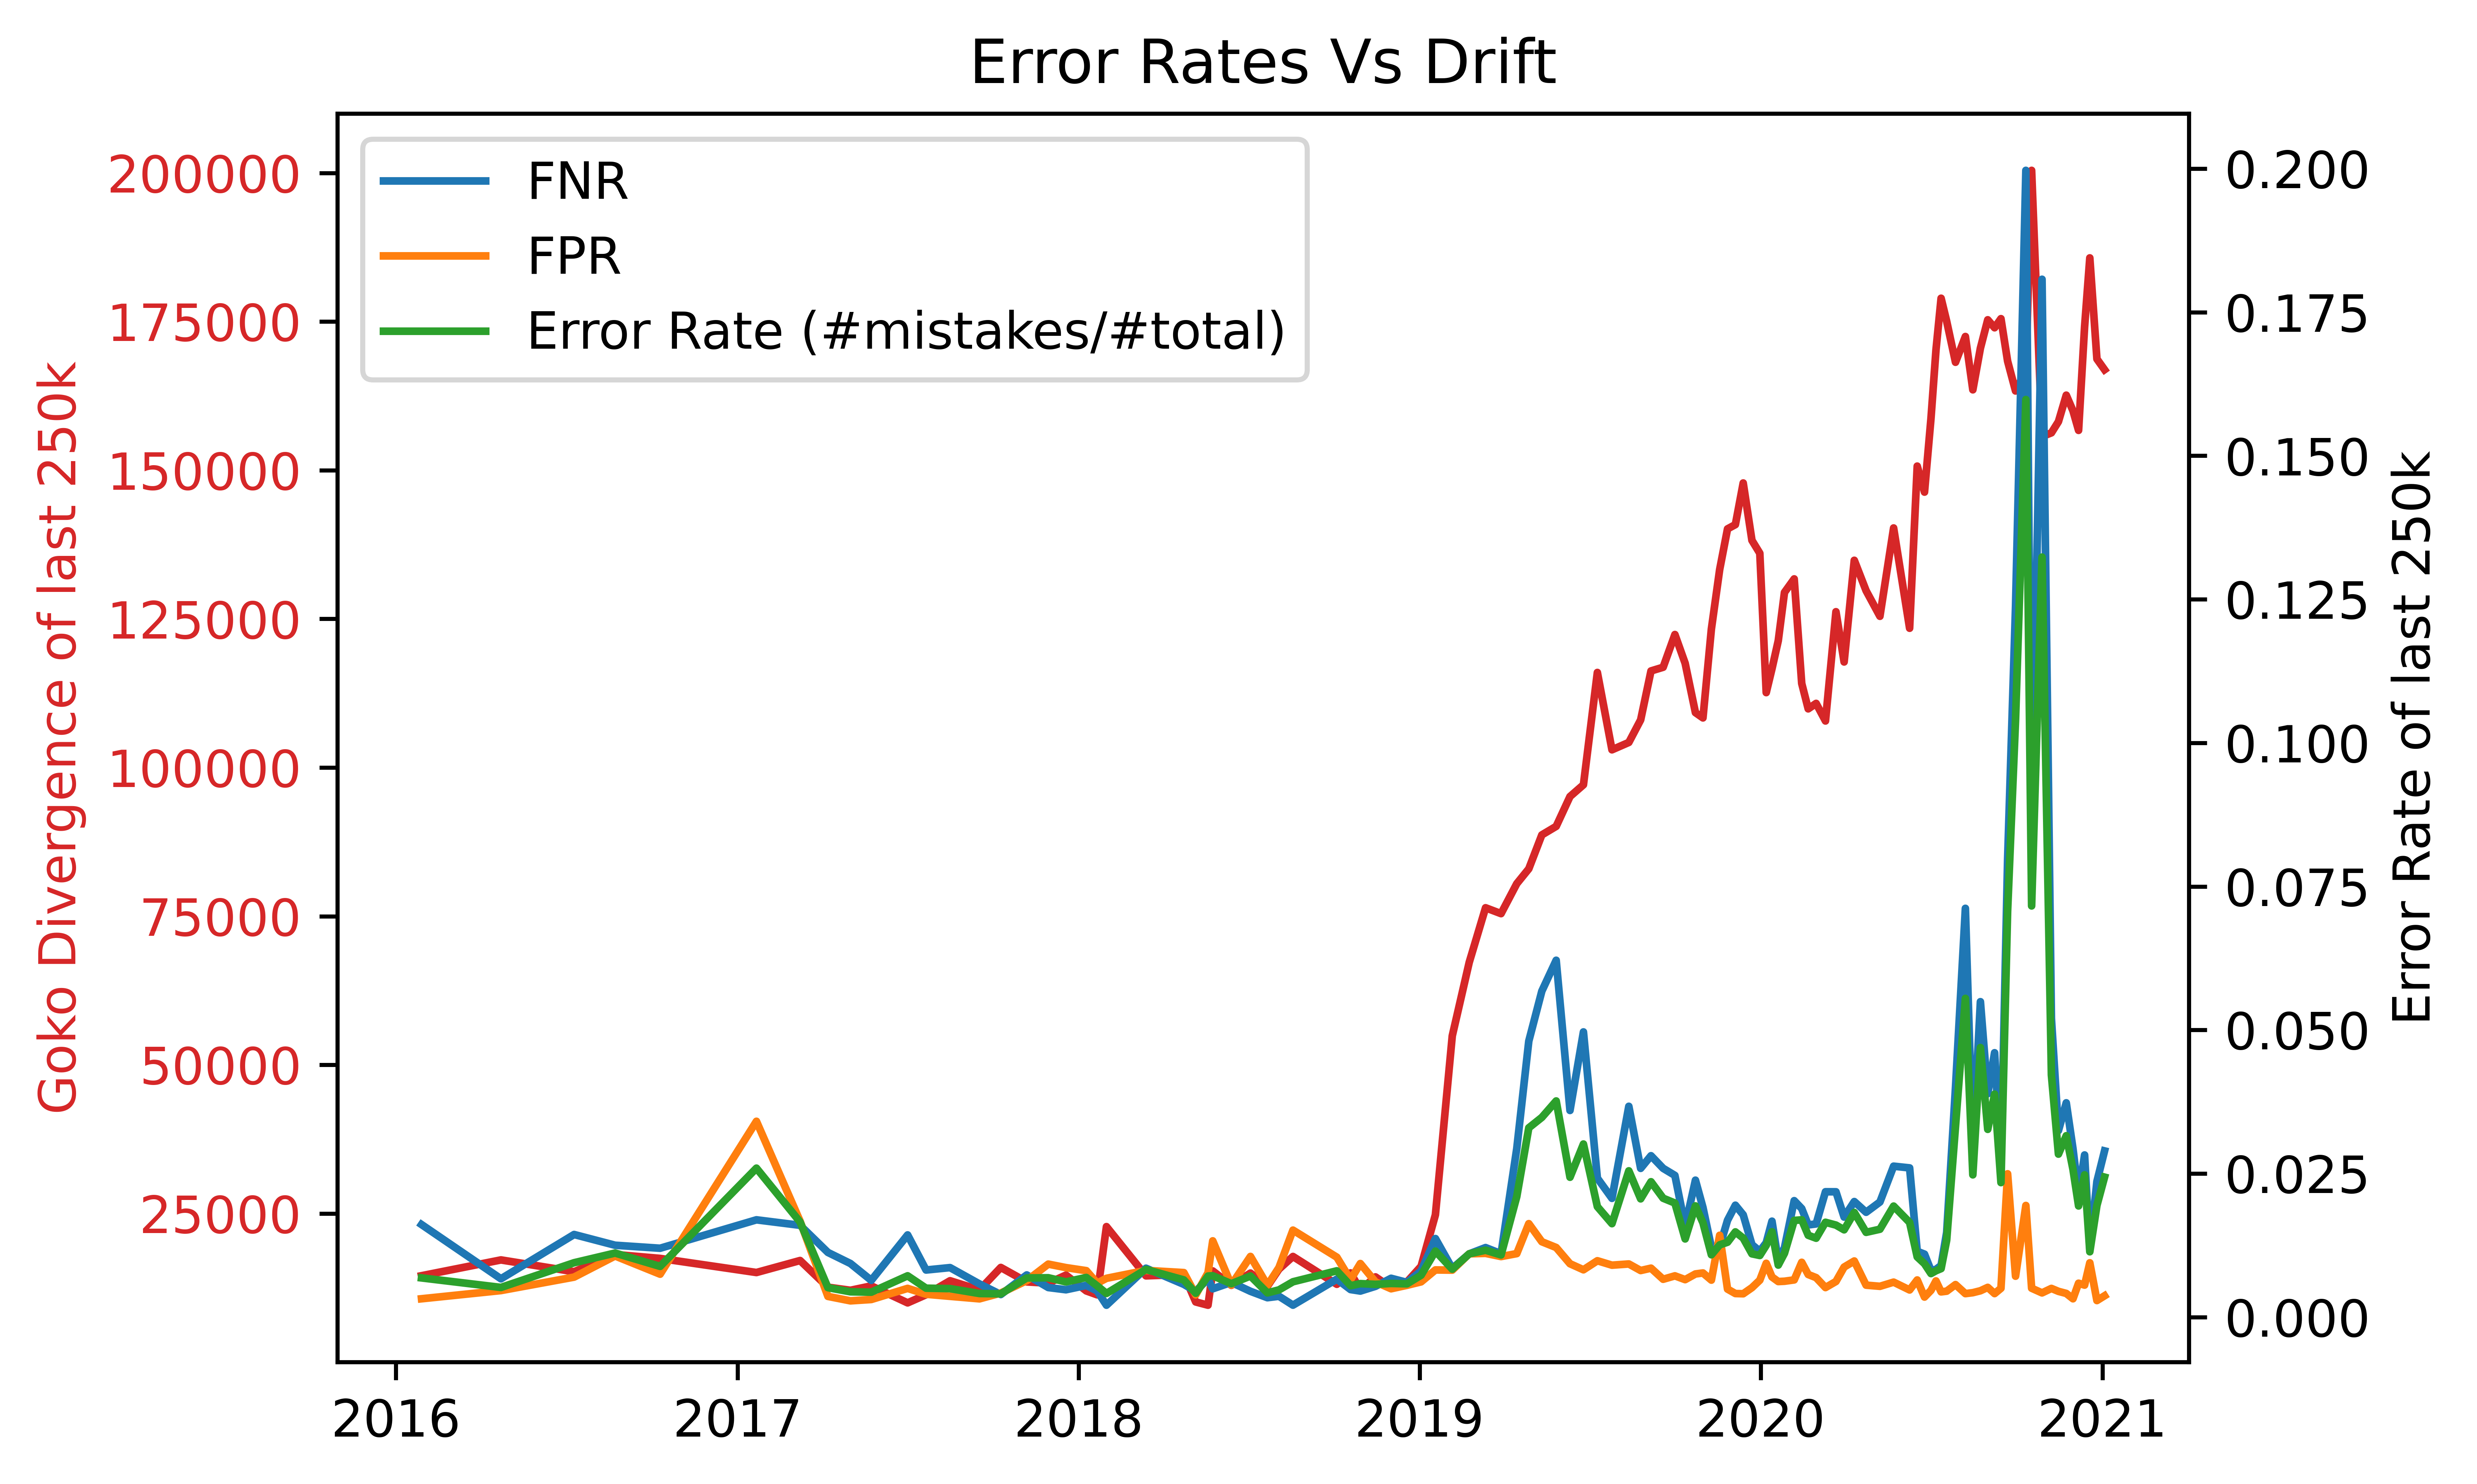
\includegraphics[scale=0.5]{overall_vs_error.png}

        \textbf{This is harder than you think.} 
    \end{center}
\end{frame}

\begin{frame}{Real Security: Understand Your Attackers}
    \begin{center}
        \begin{enumerate}
            \item \textbf{What's easy for your attacker to change?}
            \item \textbf{What's hard to change?}
            \item \textbf{What's fundamental to their objective?}
        \end{enumerate}
        \vspace{20pt}

        Spammers on social networks need a lot of accounts posting a lot of content. This behavioral data is far more reliable than content data that's easy to change.
        \vspace{10pt}
        
        Adding imports increases the on disk size of a binary, and malware authors like tiny binaries.
    \end{center}
\end{frame}

\begin{frame}{Advanced Real Security: Be a Moving Target}
    \begin{center}
        Retraining only goes so far. A bypass for a model at this point, may also be a bypass for next week's model.
        \vspace{10pt}
        
        \textbf{Constantly make new software features, and ML features.}  
        \vspace{10pt}

        When you have enough good ML features swap them out and change which ones you use each week. 
        \vspace{10pt}
        
        This policy puts an expiration date on attacks. \cite{proofpoint_cve}
    \end{center}
\end{frame}

\section{General Recommendations for ML}

\begin{frame}{For Image Based Domains}
    \textbf{In Progress}
    \vspace{10pt}

    Your data probably moves less, there's less of an incentive to mess with you. It still moves.
    \vspace{10pt}

    There's probably simpler ways of messing with your system that don't require a lot of time from a smart person with a lot of valuable knowledge.
\end{frame}

\begin{frame}{For Text Based Domains}
    \textbf{TODO}
\end{frame}

\begin{frame}[t, allowframebreaks]
\frametitle{References}
\bibliographystyle{amsalpha}
\bibliography{references.bib}
\end{frame}


\end{document}